\chapter{Designing Change-based Persistence for Models}
\label{ch:change_based_model_persistence}

This chapter presents a novel approach to change-based model persistence, including it format, requirements, design, and implementation. Potential benefits and novel capabilities as well the challenges of using a change-based format for model persistence also are highlighted in this chapter using a running example.

\section{Introduction}
\label{Introduction}

The concept of change-based persistence presented in the literature review must be translated for a modelling framework if it is to be applied for model persistence. To gain all the benefits of change-based persistence, an implementation that can save and load a model in change-based persistence must be developed first. The implementation should be able to capture all relevant changes of a model and persist them into a file. It must also be able to de-serialise changes from the file and (re)execute them in order to (re)construct the model. This research has developed a prototype of such a tool, designed to work with EMF models and meta-models.

Before exploring how change-based persistence is implemented, this chapter introduces a running example to explain the solutions proposed in this study and how model differencing and conflict detection are performed in existing tools, such as in EMF Compare \cite{emfcompare2018developer} and EMF Store \cite{emfstore2019what}. This example is used throughout this thesis to explain the proposed solutions as well.

The rest of this chapter is structured as follows. Section \ref{sec:running_example_1} introduces the running example.
Sections \ref{sec:proposed_approach} presents an overview of the proposed approach.
Section \ref{sec:prototype_implementation} discusses the prototype implementation on top of the Eclipse Modeling Framework.
The challenges of change-based model persistence are presented in
Section \ref{sec:challenges}. Section \ref{sec:conclusions_3} concludes this chapter.

\section{Running Example: Part I}
\label{sec:running_example_1}

Figure \ref{fig:class_diagram_rpg} shows three versions of an incomplete model conforming to a simplified UML-like meta-model in Figure \ref{fig:miniuml_metamodel}. The meta-model is minimalist to facilitate explaining the running example.

\begin{figure*}[h]
  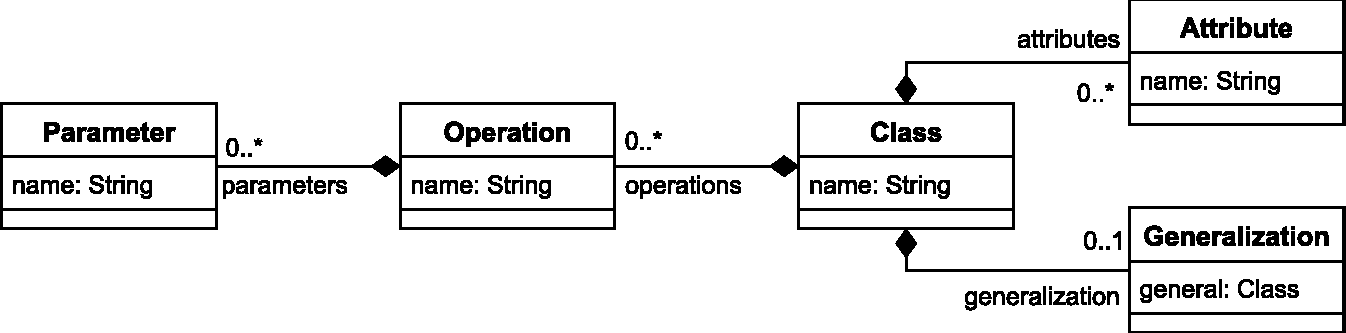
\includegraphics[width=\linewidth]{miniuml_metamodel}
  \caption{An excerpt of the UML-like meta-model of the running example in Figure \ref{fig:class_diagram_rpg}.}
  \label{fig:miniuml_metamodel}
\end{figure*}

\begin{figure*}[h]
  \centering
  \begin{subfigure}[t]{0.47\linewidth}
    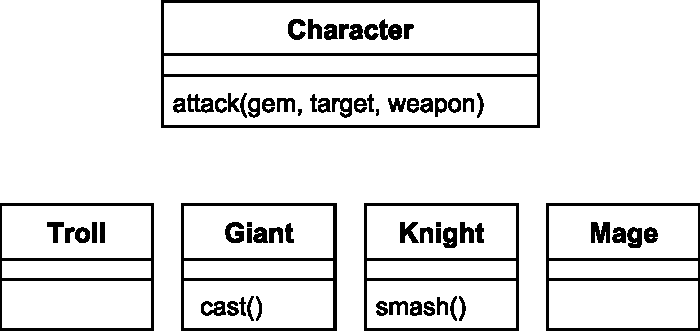
\includegraphics[width=\linewidth]{class_diagram_origin}
    \caption{original version (Jane’s version)}
    \label{fig:class_diagram_origin}
  \end{subfigure}
  \\
  \begin{subfigure}[t]{0.47\linewidth}
    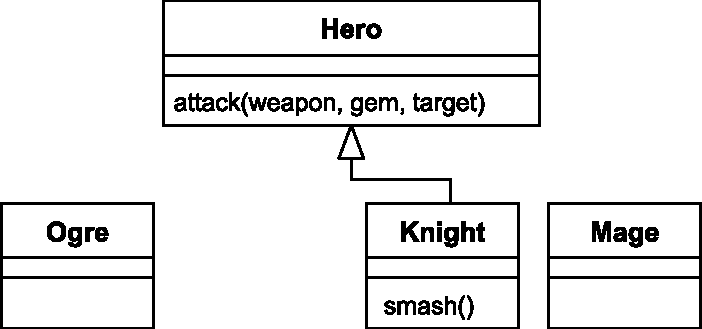
\includegraphics[width=\linewidth]{class_diagram_left}
    \caption{left version (Bob’s version)}
    \label{fig:class_diagram_left}
  \end{subfigure}
  \hfill
  \begin{subfigure}[t]{0.47\linewidth}
    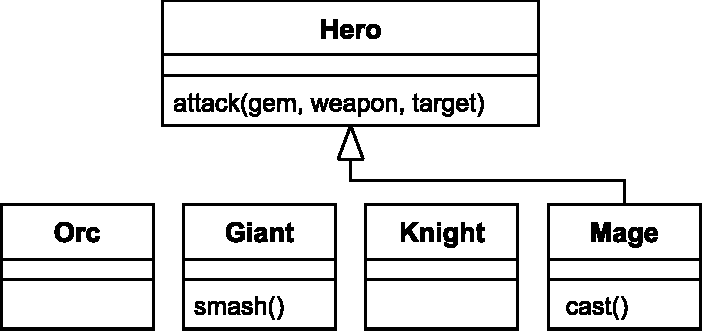
\includegraphics[width=\linewidth]{class_diagram_right}
    \caption{right version (Alice’s version)}
    \label{fig:class_diagram_right}
  \end{subfigure}
  \caption{Three incomplete class diagrams of a Role Playing Game.}
  \label{fig:class_diagram_rpg}
\end{figure*}

In this scenario, Jane has set up an initial model of a Role Playing Game (RPG) (Figure \ref{fig:class_diagram_origin}). She then assigned this work to Bob and Alice. Both Alice and Bob continued to work on the model and made some modifications, seen in Figures \ref{fig:class_diagram_left} and \ref{fig:class_diagram_right} respectively. Persisting these models in the standard XMI \cite{omg2018xmi} format produces three files as shown in Listings \ref{lst:xmimodel_origin}, \ref{lst:xmimodel_left}, and \ref{lst:xmimodel_right}. In this running example, every element has its globally unique ID. Thus, if Bob and Alice create two elements independently, they will not be allocated the same ID. For example, the generalisations that Bob and Alice added in Listings \ref{lst:xmimodel_left} and \ref{lst:xmimodel_right} have different IDs, \textsf{leftGen} and \textsf{rightGen} respectively.

\vspace{-20pt}
\begin{lstlisting}[style=xmi,caption={Simplified XMI file of the original version in Figure \ref{fig:class_diagram_origin}.},label=lst:xmimodel_origin]
<uml:Model>
  <packagedElement type=Class id="character" name="Character">
    <operation id="attack" name="attack">
      <parameter id="gem" name="gem"/>
      <parameter id="target" name="target"/>
      <parameter id="weapon" name="weapon"/>
   </operation>
  </packagedElement>
  <packagedElement type=Class id="troll" name="Troll"/>
  <packagedElement type=Class id="giant" name="Giant">
    <operation id="cast" name="cast"/>
  </packagedElement>
  <packagedElement type=Class id="knight" name="Knight">
    <operation id="smash" name="smash"/>
  </packagedElement>
  <packagedElement type=Class id="mage" name="Mage"/>
</uml:Model>
\end{lstlisting}

\vspace{-20pt}
\begin{lstlisting}[style=xmi,caption={Simplified XMI file of the left version in Figure \ref{fig:class_diagram_left}.},label=lst:xmimodel_left]
<uml:Model>
  <packagedElement type=Class id="character" name="Hero">
    <operation id="attack" name="attack">
      <parameter id="weapon" name="weapon"/>
      <parameter id="gem" name="gem"/>
      <parameter id="target" name="target"/>
    </operation>
  </packagedElement>
  <packagedElement type=Class id="troll" name="Ogre"/>
  <packagedElement type=Class id="knight" name="Knight">
    <generalization id="leftGen" general="character"/>
    <operation id="smash" name="smash"/>
  </packagedElement>
  <packagedElement type=Class id="mage" name="Mage"/>
</uml:Model>
\end{lstlisting}

\vspace{-20pt}
\begin{lstlisting}[style=xmi,caption={Simplified XMI file of the right version of Figure \ref{fig:class_diagram_right}.},label=lst:xmimodel_right]
<uml:Model>
  <packagedElement type=Class id="character" name="Character">
    <operation id="attack" name="attack">
      <parameter id="gem" name="gem"/>
      <parameter id="weapon" name="weapon"/>
      <parameter id="target" name="target"/>
    </operation>
  </packagedElement>
  <packagedElement type=Class id="troll" name="Orc"/>
  <packagedElement type=Class id="giant" name="Giant">
    <operation id="smash" name="smash"/>
  </packagedElement>
  <packagedElement type=Class id="knight" name="Knight"/>
  <packagedElement type=Class id="mage" name="Mage">
    <generalization id="rightGen" general="character"/>
    <operation id="cast" name="cast"/>
  </packagedElement>
</uml:Model>
\end{lstlisting}

An alternative way to persist these three models would be to persist the sequence of all changes through which they were constructed, not to persist their state. This approach was first introduced in \cite{DBLP:conf/models/YohannisKP17}, and it is illustrated in the next section. This example is extended in Section \ref{sec:runnnig_example_continue} to facilitate explaining the change-based model differencing proposed in this research.

\section{Proposed Approach}
\label{sec:proposed_approach}

To illustrate the proposed approach, Listing \ref{lst:xmimodel_left} shows a state-based representation of Bob’s model in Figure \ref{fig:class_diagram_left} in (simplified) XMI, and Listing \ref{lst:cbp_left_full} shows the proposed equivalent change-based representation of the same model. Instead of persisting a snapshot of the model’s state, the representation of Listing \ref{lst:cbp_left_full} captures the complete sequence of change events (create/set/add/move/remove/delete) that were performed on the model since its creation, organised in editing sessions. There are two editing session in the case of this model. The session at line 1 marks the editing made by Jane until line 29. Replaying these changes produces Jane’s model in Figure \ref{fig:class_diagram_origin}. The rest of the change events are the modification performed by Bob on Jane’s model. Replaying all the changes, both Jane’s and Bob’s changes, produces the same state as the one captured in Listing \ref{lst:xmimodel_left} or Figure \ref{fig:class_diagram_left}. Thus, we can conclude that the proposed change-based representation carries at least as much information as the state-based representation.

\vspace{-20pt}
\begin{lstlisting}[style=eol,float=tp,escapechar=|,caption={The complete change events of Bob’s model in Figure \ref{fig:class_diagram_left}.},label=lst:cbp_left_full]
session "Jane-01"
create character type Class
set character.name from null to "Character"
create attack type Operation
set attack.name from null to "attack"
add attack to character.operations at 0
create gem type Parameter
set gem.name from null to "gem"
add gem to attack.parameters at 0
create target type Parameter
set target.name from null to "target"
add target to attack.parameters at 1
create weapon type Parameter
set weapon.name from null to "weapon"
add weapon to attack.parameters at 2
create troll type Class
set troll.name from null to "Troll"
create giant type class
set giant.name from null to "Giant"
create cast type Operation
set cast.name from null to "smash"
add cast to giant.operations at 0
create knight type Class
set knight.name from null to "Knight"
create smash type Operation
set smash.name from null to "smash"
add smash to knight.operations at 0
create mage type Class
set mage.name from null to "Mage"
session "Bob-01"
create leftGen type Generalization
set leftGen.general from null to character
set troll.generalization to leftGen
set character.name from "Character" to "Hero"
unset troll.generalization from leftGen to null composite l1
set knight.generalization to leftGen composite l1
move target in attack.parameters from 1 to 2
unset cast.name from "cast" to null composite l2
remove cast from giant.operations at 0 composite l2
delete cast composite l2
unset giant.name from "Giant" to null composite l2
delete giant composite l2
set troll.name from "Troll" to "Ogre"
\end{lstlisting}

Such a representation is particularly suitable to identify the changes of the model since the last version. For example, if we can identify that changes recorded for the previous version came before editing session \textsf{Bob-01} (lines 1–29) of the model, we can readily identify the changes that were made to the model since then (i.e. in session \textsf{Bob-01}—lines 30–43) instead of having to rediscover them through expensive state-based model differencing.

For the sake of readability, the format of change-based persistence presented in Listing \ref{lst:cbp_left_full} is a simplified version. The real format is in XML-like-format (Appendix \ref{lst:class_diagram_left_cbpfile}). For example, change event \textsf{session "Jane-01"} is persisted as:

\textsf{<session ID="Jane-01" time="20190923181841687GMT"/>}

and \textsf{set character.name from null to "Character"} is persisted as:

\textsf{<set-eattribute eclass="Class" name="name"
  target = "character">
  <old-value literal=null/>
  <value literal = "Character"/>
  </set-eattribute>}.

Change events that have been persisted to a change-based persistence file cannot be altered or removed. They are immutable. Only new change events can be appended to the file.

%\section{Requirements}
%\label{sec:requirements}
%From the literature review and the text-based change summaries in the above listings, a number of requirements have been gathered as guidance for designing the implementation of change-based persistence.
%\begin{enumerate}
% \item[R1] The implementation should be able to listen and collect change events when a model is modified.
% \item[R2] It should conform to model and meta-model infrastructure of the Eclipse Modeling Framework.
% \item[R3] A change event should contain necessary information, such as change event type (add, remove, delete, create, set, unset, composite), element (class and ID), feature (name and type), value (literal or object), and index (from and to), so that when replaying them orderly an equivalent model is constructed.
% \item[R4] The implementation should be able to append change events into a change-based model file as well as to (re)load them from the file by replaying all the change events.
%\end{enumerate}

\section{Prototype Implementation}
\label{sec:prototype_implementation}

A prototype \cite{epsilonlabs2019emfcbp} of the change-based model persistence format (EMF CBP) has been implemented using the model-element level change notification facilities provided by the Eclipse Modeling Framework. In that implementation, the prototype uses a subclass of EMF’s \textsf{EContentAdapter} (\textsf{ChangeEventAdapter}) to receive and record \textsf{Notification} events produced by the framework for every model-element-level change.

\begin{figure*}[th]
  \centering
  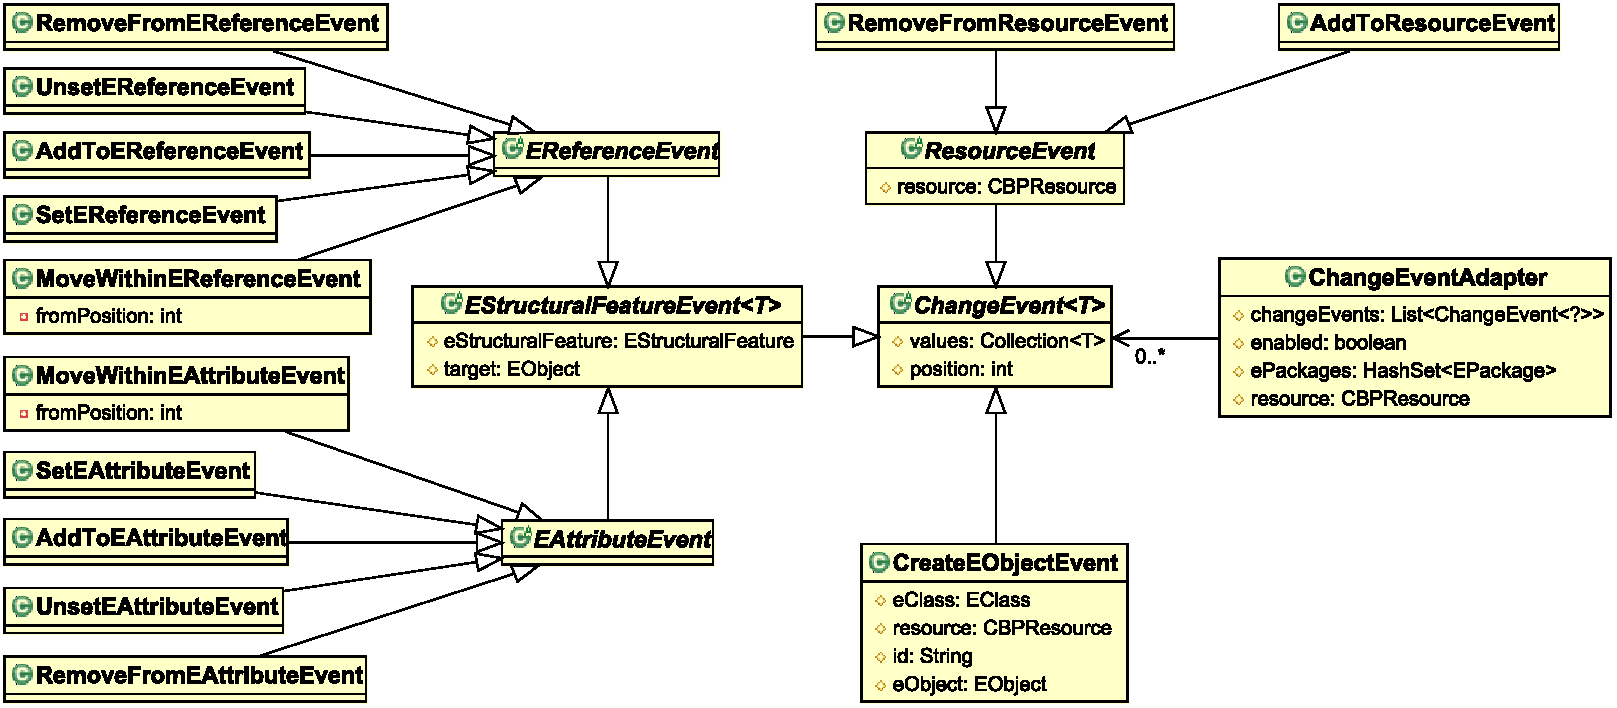
\includegraphics[width=\linewidth]{events}
  \caption{Event classes to represent changes of models.}
  \label{fig:events}
\end{figure*}

Since not all change events are relevant to change-based persistence (e.g. EMF also produces change notifications when listeners/adapted are added/removed from the model), we have defined a set of event classes to represent events of interest. The event classes are depicted in Figure \ref{fig:events} as subclasses of the \textsf{ChangeEvent} abstract class.

EMF has dedicated classes to express the graph structure of a model. For instance, \textsf{EStructuralFeature} can be \textsf{EReference} or \textsf{EAttribute}, it can have a single value or multiple values (e.g., Integer, String), the value(s) of \textsf{EStructuralFeature} can be a \textsf{EObject} or primitive, the \textsf{EReference} can be a containment or non-containment. These characteristics drive the design of the prototype to have different subclasses of \textsf{ChangeEvent}, and they also decide which attributes and methods should be defined in the class.

The \textsf{ChangeEvent} class has a multi-valued \textsf{values} attribute, which can accommodate both single-valued (e.g. set/add) or multi-valued events (e.g. addAll/removeAll). \textsf{ChangeEvent} can also accommodate different types of values, such as \textsf{EObject}s for \textsf{EReferenceEvents} and primitive values (e.g. Integer, String) for \textsf{EAttributeEvents}. The \textsf{ChangeEvent} class also has a position attribute to hold the index of an \textsf{EObject} or a literal when they are added to a \textsf{Resource}, \textsf{EReference}, or \textsf{EAttribute} with multiple values.

Every time an \textsf{EObject} is added to the model, a globally unique ID is assigned to the \textsf{EObject}, and a \textsf{CreateEObjectEvent} and an \textsf{AddToResourceEvent} are recorded. When an EObject is deleted, or moved to a containment \textsf{EReference} elsewhere in the model, a \textsf{RemoveFromResourceEvent} is recorded.

\begin{lstlisting}[style=java,caption={Simplified Java code to handle notification events.},label=lst:javacode]
public class ChangeEventAdapter extends EContentAdapter {
  ...
  @override
  public void notifyChanged(Notification n) {
  ...
  switch (n.getEventType()) {
    ... // other events
    case Notification.UNSET: {
      if (n.getNotifier() instanceof EObject) {
        EStructuralFeature feature = (EStructuralFeature) n.getFeature();
        if (feature instanceof EAttribute) {
          event = new UnsetEAttributeEvent();
        } else if (feature instanceof EReference) {
          event = new UnsetEReferenceEvent();
        }
      } break;
    }
    ... // other events
\end{lstlisting}	

The \textsf{ChangeEventAdapter} receives EMF change notifications in its \textsf{notifyChanged()} method and filters and transforms them into appropriate change events. As an example of how notifications are filtered and transformed, Listing \ref{lst:javacode} shows how the prototype handles \textsf{Notification.UNSET} events, based on the type of the feature that was changed. That is, an \textsf{UnsetEAttributeEvent} is instantiated if the feature of the notifier is an \textsf{EAttribute}, or an \textsf{UnsetEReferenceEvent} is created if the notifier is an \textsf{EReference}. The transformed instances are then stored in a list of events in \textsf{ChangeEventAdapter} (\textsf{ChangeEvents}) for persistence.

To integrate seamlessly with the EMF framework and to eventually support multiple concrete change-based serialisation formats (e.g. XML-formatted representation for readability and binary for performance/size), the prototype implemented a \textsf{CBPResource} abstract class that extends EMF’s built-in \textsf{ResourceImpl} class. The role of the abstract class is to encapsulate all change recording functionality while the role of its concrete subclasses is to implement serialisation and de-serialisation.
To save a model, \textsf{CBPXMLResourceImpl} persists changes in a line-based format where every change is serialised as a single-line XML document. In this way, when a model changes, the prototype can append the new changes to the end of the model file without needing to serialise the entire model again.
To load a model, \textsf{CBPXMLResourceImpl} de-serialises every line in the document as a change event and then re-executes it to reconstruct the model.
The prototype also includes a \textsf{CBPXMLResourceFactory} class that extends EMF’s \textsf{ResourceFactoryImpl} as the factory class for change-based models. Figure \ref{fig:resources} shows the relationships between these classes.

\begin{figure}[th]
  \centering
  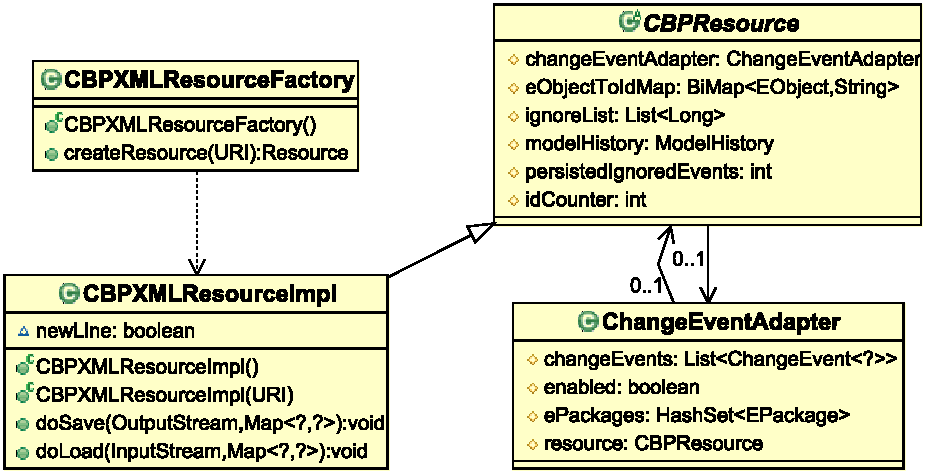
\includegraphics[width=\linewidth]{resources}
  \caption{Factory, resource, and ChangeEventAdapter classes.}
  \label{fig:resources}
\end{figure}

Listing \ref{lst:javacode_resource} shows how to use the prototype in Java code. Lines 1–8 demonstrate how to initialise and save a model using the prototype. First, the code creates an instance of \textsf{CBPResource}, \textsf{cbpResource}, using \textsf{CBPXMLResourceFactory} and specifies its file as \textsf{helloworld.cbpxml} using \textsf{URI}. The code then executes method \textsf{startNewSession} of \textsf{cbpResource}. This method adds a change event to indicate the start of the editing session as depicted at line 1 in Listings \ref{lst:cbp_origin} and \ref{lst:cbp_left}.
The code then uses \textsf{UMLFactory} to create an element, \textsf{model}, of UML2’s \textsf{Model}. The code adds element \textsf{model} into \textsf{cbpResource} and sets the name to ‘Hello World’. The code then saves the model in change-based format using method \textsf{save} and then unloads \textsf{cbpResource}. Lines 9–12 demonstrate how to replay (load) the model that had been saved and then print the name of the first element in \textsf{cbpResource}, which is expected to print “Hello World”.

\vspace{-20pt}
\begin{lstlisting}[style=java,caption={An example how to use \textsf{CBPResource} in Java code.},label=lst:javacode_resource]
/* initialise, save, and unload */
CBPResource = (CBPResource) (new CBPXMLResourceFactory()).createResource(URI.createFileURI("helloworld.cbpxml"));
cbpResource.startNewSession("Initial");
Model = UMLFactory.eINSTANCE.createModel();
cbpResource.getContents().add(model);
model.setName("Hello World");
cbpResource.save(null);
cbpResource.unload();

/* load and print */
cbpResource.load(null);
model = (Model) cbpResource.getContents().get(0);
System.out.println(model.getName()); // expected output: "Hello World"
\end{lstlisting}

%\section{Benefits and Novel Capabilities}
%\label{sec:benefits_and_novel_capabilities}
%This section highlights some of the benefitsnovel capabilities of the prototype.
%
%\begin{itemize}
%\item With appropriate tool support, modellers will be able to ‘replay’ (part of) the change history of a model (e.g. to understand design decisions made by other developers, for training purposes). In state-based approaches, this can be partly achieved if models are stored in a version control repository (e.g. Git). However, the granularity would be at the commit level only.
%\item By analysing models serialised in the proposed representation, modelling language and tool vendors will be able to develop deeper insights into how modellers use these languages/tools in practice. They can then use this information to guide the evolution of the language/tool. An early work for this case is in \cite{polack2019towards}.
%\item By attaching additional information to each session (e.g. the ID of the developer, references to external documents/URLs), sequences of changes can be traced back to the developer that made them or to the requirements/bug reports that triggered them.
%\item Persisting changes to large models after an editing session will be significantly faster than serialising the entire state of the model, as only changes made during the session will need to be appended to the model file. The evaluation of this benefit can be found in Chapters \ref{ch:optimised_loading} and \ref{ch:hybrid_model_persistence} of this thesis.
%\item The performance and precision of model differencing and conflict detection can be substantially improved, particularly for large models with shared editing histories. The evaluation of this benefit can be found in Chapters \ref{ch:model_differencing} and \ref{ch:conflict_detection} of this thesis.
%\item Using a text file to persist changes of a model allows common text-oriented version controls, such as Git and SVN, to be used for model versioning. Text-oriented version controls are not supported by EMF Store—an existing implementation of change-based persistence of EMF models—which uses its own mechanism to version models.
%\end{itemize}

\section{Challenges}
\label{sec:challenges}
This section highlights the challenges that come from adopting change-based persistence. As was mentioned in the literature review, change-based persistence also comes with a number of challenges, such as (1) loading overhead and (2) fast-growing model files, which can hold back the delivery of its potential benefits. Addressing these challenges surely facilitates its adoption.

For the first challenge, persisting changes to large models is expected to be much faster and resource-efficient than state-based approaches, since loading models into memory by naïvely replaying the entire change history is expected to have a significant overhead. This work has addressed this challenge by proposing two solutions that reduce the cost of change-based model loading. The first solution is to record and ignore events that are later overridden or cancelled out by other events. That solution can be found in Chapter \ref{ch:optimised_loading}. The second solution is a proposed hybrid model persistence format that uses change-based and state-based persistence together. In that solution, changes applied to a model are persisted into both change-based and state-based representations, but the model is loaded from the stated-based persistence. In that way, it avoids replaying the change events. This solution is discussed in Chapter \ref{ch:hybrid_model_persistence}.

In the second challenge—fast-growing model files—persisting a model in a change-based format means that the size of its file grows significantly faster during the model’s evolution than it does in its state-based counterpart. This challenge has not been addressed in this research, and must be considered in future work. Nevertheless, this research recommends two solutions. Use sound change-compression operations (e.g. remove older/unused information) to reduce the size of a model in a controlled way, or develop  a compact textual format that will minimise the space required to record a change. (A textual line-separated format is desirable to maintain compatibility with file-based version control systems.)

\section{Conclusions}
\label{sec:conclusions_3}
Through persisting models’ change history, this research aims to enable high-performance model differencing and conflict detection in collaborative development settings. This study has translated the concept of change-based persistence into an implementation in a modelling framework, which can be used to persist models.

In this chapter, a running example was introduced. This example is used throughout this thesis to explain the solutions proposed in this study. A prototype of a change-based persistence format also was presented, including its requirements and a design of the implementation that meets the requirements. Some potential benefits and novel capabilities that a change-based persistence can contribute and the challenges that might restrain delivering them also have been presented.

This chapter also has partially addressed the first research question of this study, \textbf{How can models be persisted in a change-based format, and how does change-based persistence perform, compared to state-based persistence, in terms of loading and saving models?} (RQ1). To persist models in a change-based format, a prototype has been developed. It captures relevant notifications returned by the notification facilities provided by EMF every time a change is applied to an EMF model. It then transforms the notifications into different classes of change events representing different types of changes (e.g., set, unset, add, remove, move, create, and delete) that conform to the model and meta-model infrastructure of EMF. Every captured change event is then persisted by appending it into an XML-like-formatted file when the model is saved. The model can be (re)loaded by de-serialising the file and (re)executing all the persisted change events—replaying the historical construction of the model.

